\section{Discussion}

\subsubsection{Correspondence search}
KLT vs Harris matching
\textcolor[rgb]{1,0,0}{@ Milan}

\subsubsection{Bundle-adjustment}
improvements reached
\textcolor[rgb]{1,0,0}{@Miro}

\subsubsection{Pose estimation algorithm}
We investigated pose estimation with DLT refinement after the P3P-Guess and without refinement (using the last P3P guess from RANSAC). It turned out, that very often the P3P-guess was a lot better and especially more robust then the DLT refinement. \cref{parking_result_fig_dlt} shows the estimated trajectory with DLT refinement. It is clearly worse then the P3P estimate as shown in \cref{parking_result_fig}. That's why we used the last P3P guess in our implementation.
\begin{figure*}[ht!]
    \centering
    \begin{subfigure}[t]{0.5\textwidth}
        \centering
        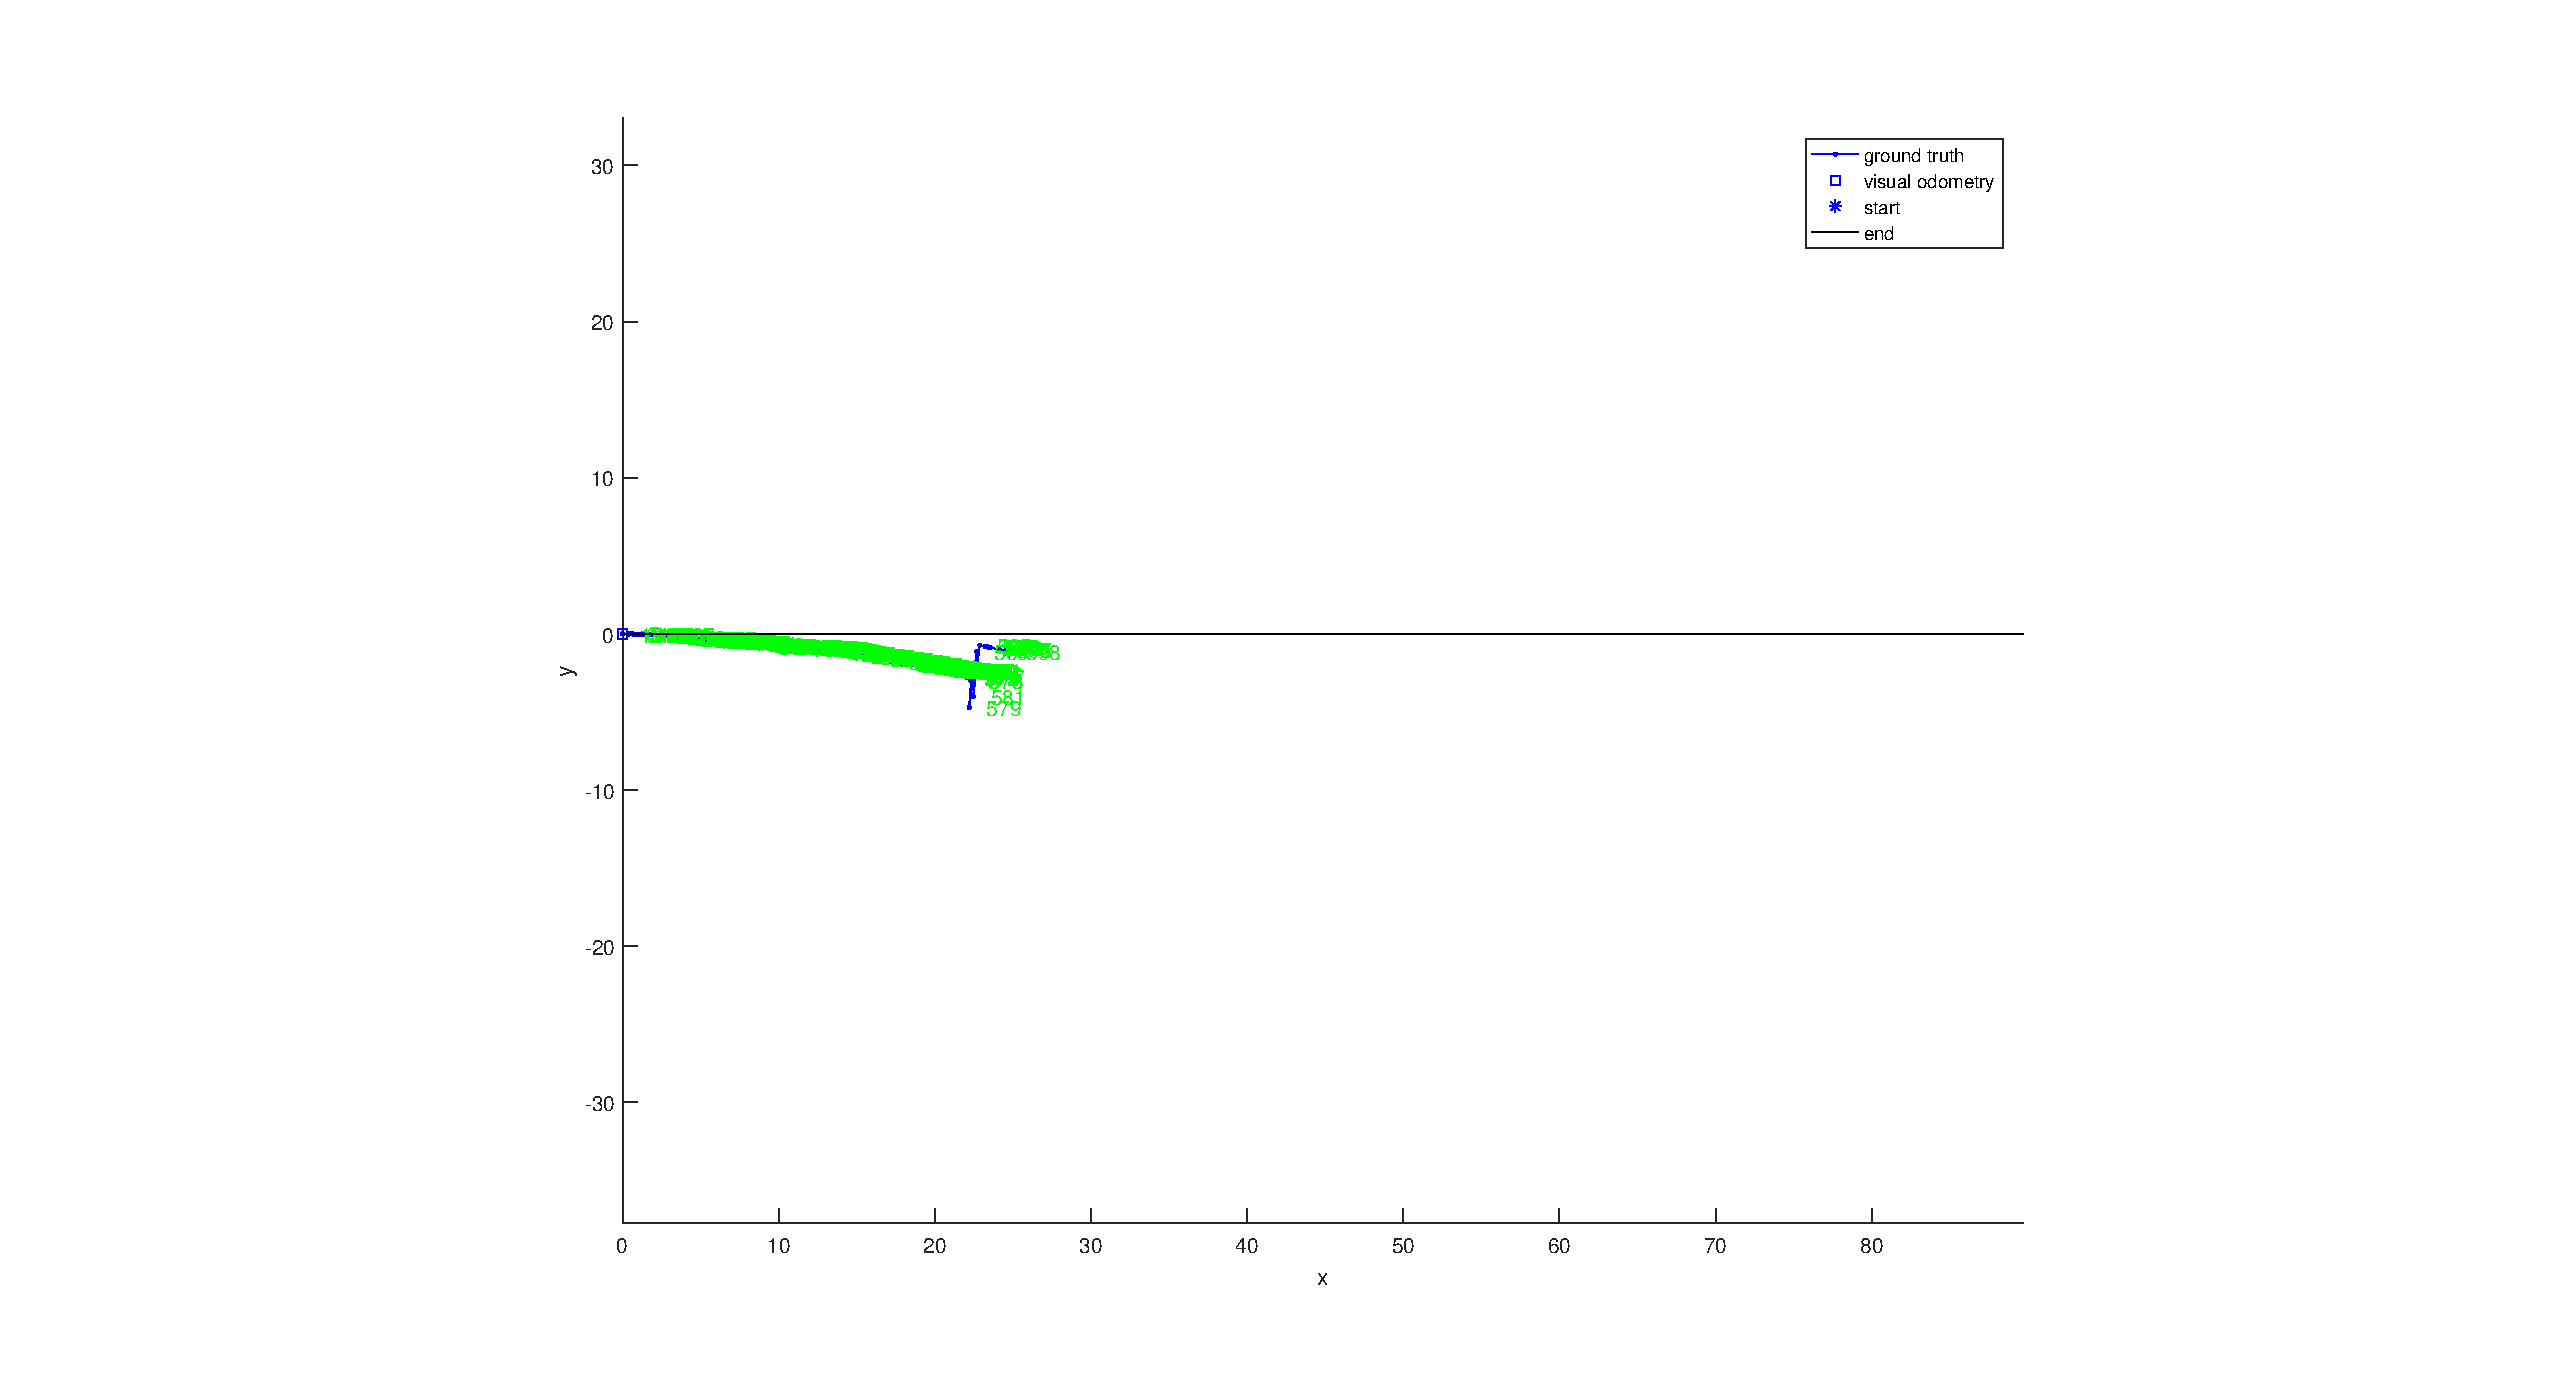
\includegraphics[height=2.7in]{results/trajectory_parking_dlt.eps} 
        \caption{Trajectory vs. ground truth}
    \end{subfigure}%
    ~ 
    \begin{subfigure}[t]{0.5\textwidth}
        \centering
        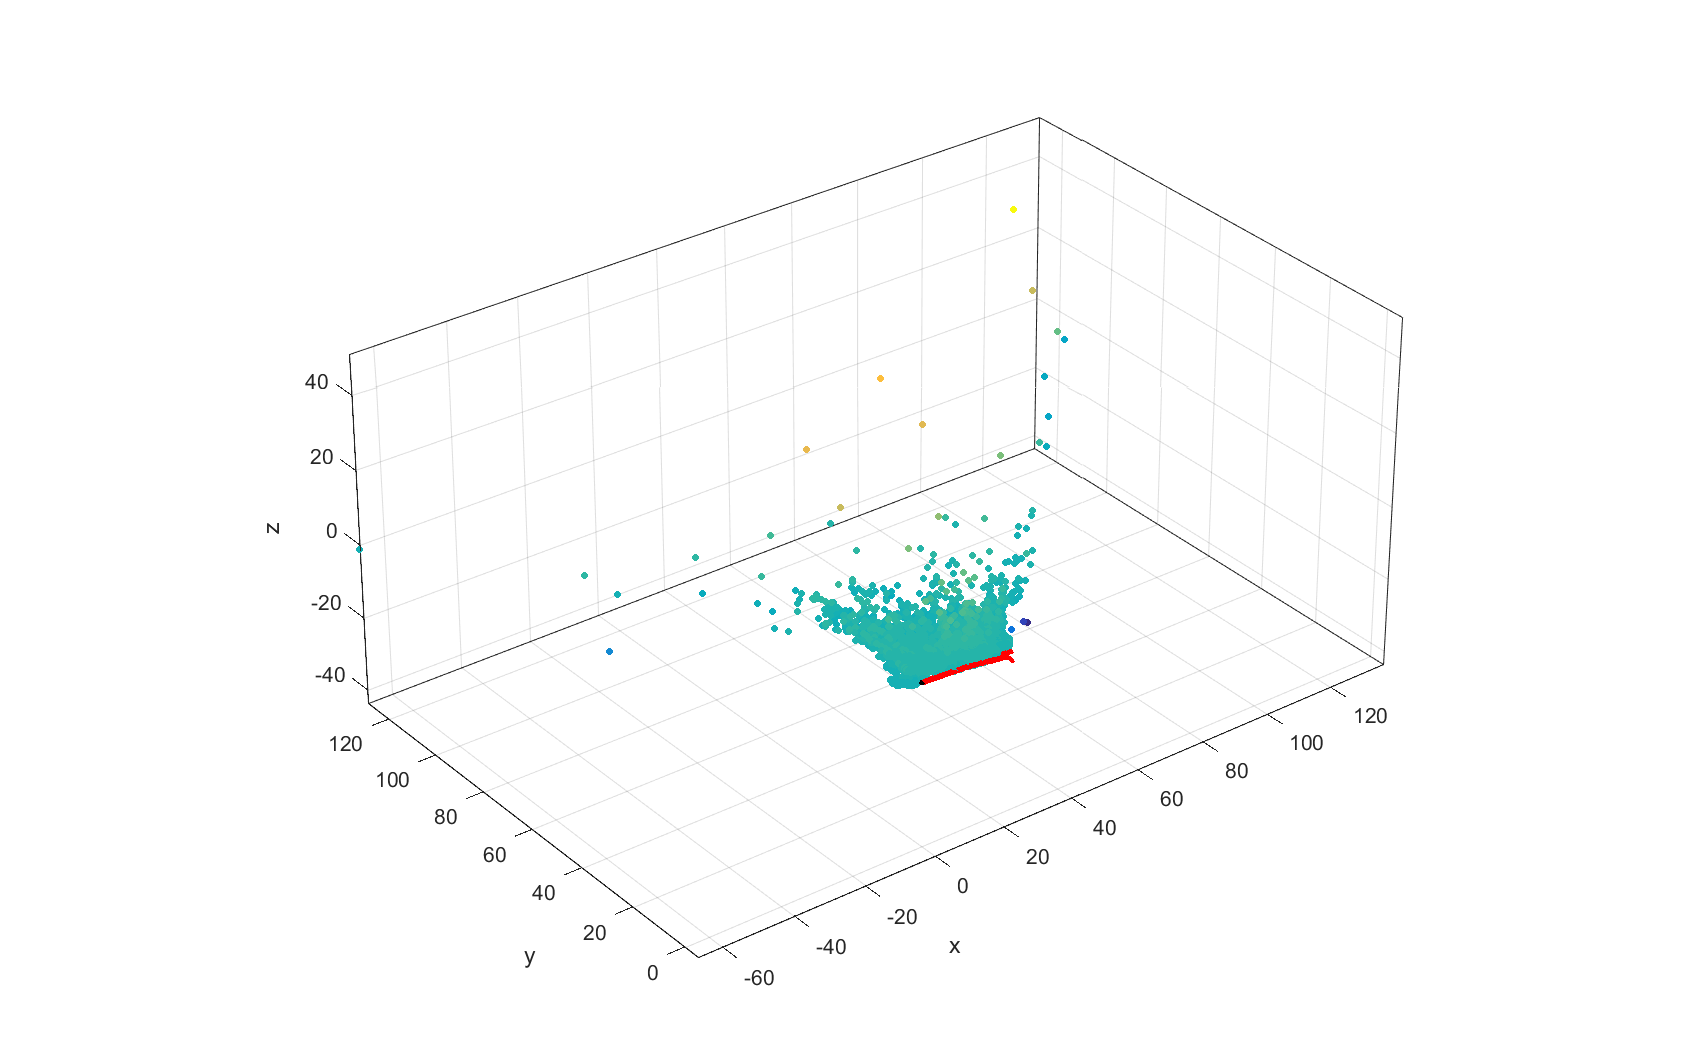
\includegraphics[height=2.7in]{results/landmarks_parking_dlt.eps}
        \caption{3D landmarks}
    \end{subfigure}
    \caption{Parking dataset results with DLT refinement}
		\label{parking_result_fig_dlt}
\end{figure*}

\subsubsection{Reinitialization}
\textcolor[rgb]{1,0,0}{@Milan}
How often does it happen? Is the result better afterwards?
